%% use
%% library(cacheSweave)
%% Sweave("unmarked.Rnw", driver = cacheSweaveDriver)


\documentclass[article,shortnames]{jss}
\usepackage{amsmath,amssymb}
\usepackage[utf8]{inputenc}
\usepackage{rotating}
\usepackage{float}

%% need no \usepackage{Sweave.sty}

\DeclareMathOperator{\logit}{logit}
\DeclareMathOperator{\Bern}{Bernoulli}
\DeclareMathOperator{\Bin}{Binomial}
\DeclareMathOperator{\Poi}{Poisson}
\DeclareMathOperator{\MN}{Multinomial}

\newcommand{\um}{\pkg{unmarked}}
\newcommand{\rlang}{\proglang{R}}
\newcommand{\scovs}{\code{siteCovs}}
\newcommand{\ocovs}{\code{obsCovs}}

\author{Ian J. Fiske\\North Carolina State University \And
  Richard B. Chandler\\ USGS Patuxent Wildlife Research Center}
\title{\pkg{unmarked}:\\
  An \proglang{R} package for Fitting Hierarchical Models of
  Wildlife Occurrence and Abundance}

\Plainauthor{Ian Fiske, Richard Chandler}
\Plaintitle{Unmarked: An R Package for Fitting Hierarchical Models of
  Wildlife Occurrence and Abundance}
\Shorttitle{\um: Analyze Wildlife Data in \proglang{R}}

\Abstract{Ecological research uses data collection techniques that are
  prone to substantial and unique types of measurement error to
  address scientific questions about species abundance and
  distribution.  These data collection schemes include a number of
  survey methods in which unmarked individuals are counted, or
  determined to be present, at spatially-referenced sites. Examples
  include site occupancy sampling, repeated counts, distance sampling,
  removal sampling, and double observer sampling.  To appropriately
  analyze these data, hierarchical models have been developed to
  separately model explanatory variables of both a latent abundance or
  occurrence process and a conditional detection process.  Because
  these models have a straightforward interpretation paralleling
  mechanisms under which the data arose, they have recently gained
  immense popularity.  The common hierarchical structure of these
  models is well-suited for a unified modeling interface.  The
  \proglang{R} package \pkg{unmarked} provides such a unified modeling
  framework, including tools for data exploration, model fitting,
  model criticism, post-hoc analysis, and model comparison.}

\Keywords{ecological, wildlife, hierarchical, occupancy, occurrence,
  distance, point count}
\Plainkeywords{ecological, wildlife, hierarchical, occupancy,
  occurrence, distance, point count}


\Address{
Ian Fiske\\
Department of Statistics\\
North Carolina State University\\
2311 Stinson Drive \\
Campus Box 8203 \\
Raleigh, NC 27695-8203 \\
E-mail: \email{ijfiske@ncsu.edu}

Richard Chandler \\
USGS Patuxent Wildlife Research Center \\
Gabrielson Lab, Room 226 \\
12100 Beech Forest Rd. \\
Laurel, MD 20708 \\
E-mail: \email{rchandler@usgs.gov}
}



\begin{document}


\section{Introduction}


\subsection{Imperfect detection and data collection in ecological research}

A fundamental goal of ecological research is to understand how environmental
variables influence spatial or temporal variation in species abundance or
occurrence.  Addressing these research questions is complicated by imperfect
detection of individuals or species.  Individuals may go
undetected when present for a variety of reasons including their proximity to
the observer, cryptic behavior, or camouflage. Thus, imperfect detection
can introduce substantial measurement error and obscure underlying
ecological relationships if ignored.

To accommodate imperfect detection of individuals or species,
ecologists have developed specialized methods to survey wildlife
populations such as site occupancy sampling, repeated counts,
distance sampling, removal sampling, and double observer sampling
\citetext{see Section~\ref{sec:models-impl-unmark} and
\citet{WilliamsEA2002} for definitions}.  This myriad of sampling methods
are all unified by a common repeated-measures type of sampling design in
which $J$ ``observations'' are made at $M$ spatial sample units during each of
$T$ seasons. As an example, Table~\ref{tab:exdata} shows a typical
repeated count dataset.

\begin{table}[h]
\begin{centering}
%\footnotesize
\begin{tabular}{lccccccc}
\hline
& \multicolumn{3}{c}{Season 1} && \multicolumn{3}{c}{Season 2} \\
\cline{2-4} \cline{6-8}
        & Visit 1 & Visit 2 & Visit 3 && Visit 1 & Visit 2 & Visit 3 \\
\hline
Site 1  & 3       & 3       & 2       && 0       & 0       & 0 \\
Site 2  & 0       & 0       & 0       && 0       & 0       & 0 \\
Site 3  & 4       & 6       & 5       && 5       & 5       & 3 \\
Site 4  & 0       & 0       & 0       && 0       & 0       & 2 \\
\hline
\end{tabular}
\caption{An example of the data structure required by \um's fitting functions.
Counts of organisms were made at $M=4$ sites during $T=2$ seasons with $J=3$
visits (``observations'') per season.}
\end{centering}
\label{tab:exdata}
\end{table}

In addition to the repeated-measures structure, there are two important
features to note about the data shown in Table~\ref{tab:exdata}.  First,
this design is often referred to as a `metapopulation design' because
the population may be regarded as an aggregation of subpopulations and
because the spatial sampling is an explicit component of the problem.
This is important because it provides a basis for modeling variation
among sites as a function of site-specific covariates, and because
metapopulation parameters such as local colonization and extinction
can be directly estimated. Second, the counts are of individuals that
may not be uniquely recognized, so although it may be possible to
determine if three individuals were detected on two different visits
(as was the case at Site 1 in Table~\ref{tab:exdata}), it is not always
possible to determine if they were the {\it same} three individuals.

Both the metapopulation design and absence of individual recognition
distinguish these data from data collected using another large suite of
ecological sampling methods known as `capture-recapture' methods. A vast number
of models have been developed for capture-recapture data, and many of them
are implemented in the software program \emph{MARK}
\citep{whiteBurnham99_MARK}. The origins of \um\ (the package and its name)
arose to fill the void of models for data from studies of unmarked
individuals involving explicit spatial sampling.

\subsection{Hierarchical models for metapopulation designs}

While many ecological studies produce data consistent with a
metapopulation design, the development and implementation of
models for inference under individual sampling protocols has
proceeded in a piecemeal fashion, without a coherent analysis
platform. Recently, however, a broad
class of hierarchical models \citetext{see \citet{royleDorazio08} for a
general treatment} has been developed that offer a unified
framework for analysis by formally recognizing that observations are
generated by a combination of (1) a \emph{state} process
determining abundance or species occurrence at each site and (2) a
\emph{detection} process that yields observations conditional on the
state process. The model for the state process describes abundance or
occurrence at each site, but due to imperfect detection, these quantities
cannot be observed directly and are regarded latent variables.

This paper introduces \um, an \rlang\ package that provides a
unified approach for fitting this broad class of hierarchical
models developed for sampling biological populations.  Inference in \um\
is based on the integrated likelihood wherein the latent state
variable is marginalized out of the conditional likelihood.


\subsection[Scope and features of unmarked]{Scope and features of \pkg{unmarked}}

\um\ provides tools to assist researchers with every step of the analysis
process, including data manipulation and exploration, model fitting, post-hoc
analysis, model criticism, and model selection.  \um\ provides a growing list
of model-fitting functions designed for specific
sampling methods.  The fitting functions each find the maximum likelihood
estimates of parameters from a particular model
(Section~\ref{sec:fitting-models}) and return an object that can be easily
manipulated.  Methods exist for performing numerous post-hoc analyses such as
requesting linear combinations of parameters, back-transforming parameters to
constrained scales, determining confidence intervals, and evaluating goodness
of fit.  The model specification syntax of the fitting functions was designed
to resemble the syntax of \rlang's common fitting functions such as \code{lm}
for fitting linear models.

Although there is existing software for fitting some of these models
\citetext{e.g., \citet{Hines2002}}, there are a number of advantages to a unified
framework within \rlang.  Many researchers are already familiar with \rlang\
and use its powerful data manipulation and plotting capabilities.  Sometimes
many species are analyzed in tandem, so that a common method of aggregating
and post-processing of results is needed, a task easily accomplished in
\rlang.  Unlike other available software, \um\ makes it possible to map
habitat-specific abundance and species distributions when combined with
\rlang's GIS capabilities.  Another important advantage of \um's approach is
that researchers can simulate and analyze data within the same
computational environment.  This work flow permits simulation studies for power
analysis calculations or the effectiveness of future sampling designs.  All of
this is made much simpler by analyzing the data within \rlang, and using a
single environment to complete all phases of the analysis is much less
error-prone than switching between applications.

In this paper, Section~\ref{sec:models-impl-unmark} gives a brief summary of
many of the models \um\ is capable of fitting.
Section~\ref{sec:unmarked-usage} describes general \um\ usage aided by a
running data example.

\section[Models implemented in unmarked]{Models implemented in \um}
\label{sec:models-impl-unmark}

The list of models implemented in \um\ continues to grow as new models are
developed. Table~\ref{tab:models} shows the models available as of version
0.9-0.  Rather than describe each fitting function in detail, this section
provides a summary of several of the most common sampling techniques and how
\um\ can be used to model the resulting data.

\begin{table}[ht] \small
%\begin{sidewaystable} \small
%\begin{tabular}{lp{2cm}cc}
\centering
\begin{tabular}{p{4cm} c c c }
\hline
\textbf{Model} & \textbf{Fitting} & \textbf{Data} & \textbf{Citation} \\
               & \textbf{function}&& \\ \hline
Occupancy from detection / non-detection data & \code{occu} & unmarkedFrameOccu & \citealt{MacKenzie2002} \\
Abundance from detection / non-detection data & \code{occuRN}& unmarkedFrameOccu & \citealt{Royle2003} \\
Abundance from repeated counts &\code{pcount}& unmarkedFramePCount & \citealt{Royle2004} \\
Abundance from distance sampling &\code{distsamp}& unmarkedFrameDS & \citealt{Royle2004b} \\
Abundance from multinomial counts &\code{multinomPois}& unmarkedFrameMPois & \citealt{Royle2004a} \\
Abundance from repeated multinomial counts &\code{gmultmix} & unmarkedFrameGMM & \citealt{chandlerEA_TempEm} \\
Multi-season occupancy &\code{colext}& unmarkedMultFrame & \citealt{MacKenzie2003} \\
Multi-season abundance & \code{pcountOpen} & unmarkedFramePCO & \citealt{DailMadsen2011} \\
\hline
\end{tabular}
\caption{Models currently handled by unmarked along with their associated
  fitting functions (Section~\ref{sec:models-impl-unmark}) and data
  type (Section~\ref{sec:data-requirements}).}
\label{tab:models}
%\end{sidewaystable}
\end{table}

\subsection{Site occupancy models}

\subsubsection{Single season site occupancy model}
\label{sec:occ}

An important state variable in ecological research is species occurrence
(or `site occupancy'), say $Z_{i}$, a binary state variable such that
$Z_{i}=1$ if site $i$ is occupied by a species and $Z_{i}=0$ otherwise.
Much interest is focused on estimating functions of species occurrence
(e.g., number of occupied sites) or to identify factors that are
associated with changes in the probability of a site being
occupied, i.e., $\psi  = \Pr(Z_{i}=1)$. To estimate these parameters,
researchers employ a sampling design, whereby surveyors visit a sample of $M$
sites and record the binary response $Y_{ij}$ of species detection ($Y=1$) or
non-detection ($Y=0$) during $j=1,\ldots,J_{i}$ visits to the $i$th site
during a `season' \citep{MacKenzie2002}.
A key feature of species occurrence surveys is that false absences are
possible, so that a species might go undetected ($Y_{ij} =0$) even if it is
present ($Z_{i} = 1$). The detection probability parameter $p$ accounts for this
observation process, and is defined as the
probability of detecting a species that is present.

The key assumptions made when modeling these data are that the occupancy
state at a site remains constant throughout the season and repeated visits at
a site are independent.  In order to meet the first assumption, a
season will generally be a very short time frame, such as
a few months during a breeding season, or even a few minutes if repeated
visits are made in quick succession.  Replicate samples (i.e., $J>1$) are
necessary to obtain information about the detection rate separate from
the occupancy rate.

The following hierarchical model describes the joint distribution of the
observations conditional on the latent occupancy state, and the marginal
distribution of the latent occupancy state variable:
\begin{gather}
Z_i \sim \Bern(\psi) \text{\quad for $i=1,2,\dots,M$} \notag \\
Y_{ij}|Z_i \sim \Bern(Z_i p)\text{\quad for $j=1,2,\dots,J_{i}$} \notag
\end{gather}
Removing the latent $Z$ variables by marginalization yields the likelihood:

\begin{equation}
L(\psi, p | \left\{Y_{ij}\right\}) =
 \prod_{i=1}^{M} \left\{
    \prod_{j=1}^{J_i}
      \left(p^{Y_{ij}}(1-p)^{1-Y_{ij}}\right)
          \psi + I(Y_{i.}=0)(1-\psi) \right\},
\end{equation}

where $I(.)$ is the indicator function taking the value 1 if its argument is
true, and 0 otherwise. The model and likelihood are easily generalizable to
accommodate covariates on detection probability or occupancy.
Variables that are related to the occupancy state are modeled as

\begin{gather}
  \logit(\psi_i) = \mathbf x_i' \mathbf \beta, \notag
\end{gather}
where $\mathbf x_i$ is a vector of site-level covariates and $\mathbf \beta$
is a vector of their corresponding effect parameters.  Similarly, the
probability of detection can be modeled with
\begin{gather}
  \logit(p_{ij}) = \mathbf v_{ij}' \mathbf \alpha, \notag
\end{gather}
where $\mathbf v_{ij}$ is a vector of observation-level covariates and
$\mathbf \alpha$ is a vector of their corresponding effect parameters.
Examples of site-level covariates include habitat characteristics such as
vegetation height. Observation-level covariates could include time of day,
date, wind speed, or other factors that might affect detection probability.
The function \code{occu} implements this model.


\subsubsection{Multi-season site occupancy model}

Sometimes the study objective is to understand the dynamics of the
occupancy state over time. To obtain such information researchers conduct
repeated occupancy studies (see Section~\ref{sec:occ}) at the same sample of
sites over consecutive seasons \citep{MacKenzie2003} and seek to estimate
probabilities of colonization ($\gamma$) and extinction
($\epsilon$), where colonization is the change of an unoccupied
site to occupied and extinction if the change of an occupied site to
unoccupied.  If the occupancy status is assumed to evolve according to
a Markov process, then a 2-state finite hidden Markov model describes
these data.  Let $Y_{ijt}$ denote the observed species occurrence
status at visit $j$ during season $t$ to site $i$.  Then
\begin{gather}
  Z_{i1} \sim \Bern(\psi) \notag \\
  Z_{it} \sim
  \begin{cases}
    \Bern(\gamma_{t-1}) & \text{if $Z_{i(t-1)} = 0$} \notag \\
    \Bern(1-\epsilon_{t-1}) & \text{if $Z_{i(t-1)} = 1$}
  \end{cases}, \\
  \text{for $t=2,3,\dots,T$} \notag \\
  Y_{ijt} | Z_{it} \sim \Bern(Z_{it} p) \notag
\end{gather}

This model generalizes the single season site occupancy model by relaxing the
population closure assumption. To define the likelihood of this model,
let $\phi_0 = (\psi, 1-\psi)$ and

\begin{equation}
  \theta_{{\bf Y_{it}}} =
  \begin{pmatrix}
    \prod_{j=1}^{J} p I(Y_{ijt}=0)(1-p) \\
    I(\sum_{j=1}^{J} Y_{ijt}=0). \notag\\
  \end{pmatrix}
\end{equation}

Furthermore, let the matrix of one-step Markov transition probabilities be

\begin{equation}
  \Phi_t =
  \begin{pmatrix}
    1-\epsilon & \epsilon \\
    1-\gamma & \gamma \notag\\
  \end{pmatrix}
\end{equation}

The likelihood is then given by

\begin{equation}
L(\psi,\epsilon,\gamma,p | \left\{Y_{ijt}\right\}) =
 \prod_{i=1}^{M} \left\{
    \phi_0 \left\{ \prod_{t=1}^{T-1} \Phi_t \theta_{Y_{it}}
        \right\} \theta_{Y_{iT}} \right\},
\end{equation}

which can be maximized by the \code{colext} function in \um. Again,
each of the four model parameters $\psi$, $\gamma$,
$\epsilon$, and $p$ can be modeled as functions of covariates on the logit
scale.


\subsection{Abundance models}

\subsubsection{Repeated count data}
\label{sec:repeated-count-data}

Occupancy is a crude summary of population structure and dynamics and in
practice considerable effort is focused on obtaining information about
abundance \citep{dorazio07}. A common sampling design for obtaining
abundance information,
analogous to the basic occupancy design described above, is to
repeatedly visit a sample of $M$ sites $J$ times and
record the number of unique individuals observed at each site.
Similar assumptions are made as with occurrence data: (1) abundance at
a site remains constant during a season and (2) counts at a site are
independent.  \citet{Royle2004} presented the following hierarchical model for
repeated count data.  Let $N_i$ be the unobserved total number of
individuals using a site and define $Y_{ij}$ as the number of individuals
observed during the $j$th visit.  Then,
\begin{gather}
\label{eq:pc2}
  N_i \sim f(\lambda, \theta) \text{\quad for $i=1,2,\dots,M$}  \notag\\
  Y_{ij}|N_{i} \sim \Bin(N_i, p)\text{\quad for $j=1,2,\dots,J_{i}$} \notag,
\end{gather}
where $\lambda_i$ is the abundance rate at site $i$ and $p$ is
the detection probability.  $f$ is
a discrete distribution with support restricted to $N_{i} \ge 0$ and
$\theta$ are extra parameters of $f$ other than the location
parameter, $\lambda$.  \um\ currently supports $f$ as Poisson or
negative binomial.  In the
negative binomial case, $\theta$ is a dispersion parameter, which is
useful when overdispersion is suspected. In the Poisson case,
the overdispersion parameter $\theta$ is constrained to equal zero.

As with the occupancy model, covariates may be included at either the
state (here, abundance) or detection levels, but abundance is modeled
through a log link to enforce its positivity constraint.
\begin{gather}
  \log(\lambda_i) = \mathbf x_i' \mathbf \beta, \notag
\end{gather}
where $\mathbf x_i$ is a vector of site-level covariates and $\mathbf \beta$
is a vector of their corresponding effect parameters.  Similarly, the
probability of detection can be modeled with
\begin{gather}
  \logit(p_{ij}) = \mathbf v_{ij}' \mathbf \alpha, \notag
\end{gather}
where $\mathbf v_{ij}$ is a vector of observation-level covariates and
$\mathbf \alpha$ is a vector of their corresponding effect parameters.

The $N_{i}$ variables are latent and so analysis is carried out based on
the integrated likelihood obtained by marginalizing each $N_{i}$ from the
conditional likelihood \citep{Royle2004b}:

\begin{equation}
L(\lambda, p | \left\{Y_{ij}\right\}) =
 \prod_{i=1}^{M}
 \left\{ \sum_{N_{i}=\max({\bf Y_i})}^{\infty}
          \left( \prod_{j=1}^{J}
     \frac{N_{i!}}{ (N_{i}-Y_{ij})!} p^{Y_{ij}}(1-p)^{N_{i}-Y_{ij}} \right)
       \frac{e^{-\lambda} \lambda^{N_i}}{N_i!} \right\}.
\end{equation}

This likelihood can be maximized using the \code{pcount} function.

The function \code{pcountOpen} implements a generalized form of this model
designed for `open' populations with temporal dynamics governed by
apparent survival and recruitment parameters \citep{DailMadsen2011}. Another
related model was described by \citet{Royle2003} and can be fit with the
\code{occuRN} function. This model estimates abundance from site occupancy
data by exploiting the link between abundance and detection probability.

\subsubsection{General multinomial-Poisson mixture model}

\label{sec:gener-mult-poiss}
Here we discuss a more general class of models that can be customized by the
user for a variety of sampling methods, the multinomial-Poisson model
\citep{Royle2004a}.   The general form of this model is
\begin{gather}
\label{eq:mp2}
  N_i \sim \Poi(\lambda) \text{\quad for $i=1,2,\dots,M$}  \notag \\
  \mathbf Y_i | N_{i} \sim \MN\left(N_i, \boldsymbol \pi \right) \notag
\end{gather}
where $N_i$ is the latent abundance at site $i$ as with the repeated
count model, and $\boldsymbol \pi=(\pi_1,\pi_2,\dots,\pi_J)'$ is
the vector of cell probabilities corresponding to the vector of counts
$\mathbf Y_{i}$.  Examples of sampling methods that produce data of
this form include removal sampling, double observer sampling,
and distance sampling. In the next sections, we discuss these specific
cases.  In general, $\boldsymbol \pi$ is
determined by the specific sampling method and
$\sum_{j} \pi_{j} \le 1$ because detection is imperfect and
$\pi_{J+1}=1 - \sum_{j} \pi_{j}$  is the probability of the species
escaping detection.

Note that the replication here is of a different
nature than in previously described models -- not over time necessarily --
but still effectively replication as far as the design goes. That is,
there are repeated measurements at each site, but with a multinomial protocol,
the replicate counts are {\it dependent} instead of independent.

To illustrate the likelihood under a multinomial observation model,
suppose that a sampling method produces a multinomial observation
with 3 observable frequencies at each site, {\it ie} $J=3$. As before,
$N_i$ are latent variables, and so inference is based on the integrated
likelihood of ${\bf Y}_{i}$ which is:

\begin{equation}
L(\lambda, p | \left\{{\bf Y}_i\right\}) =
 \prod_{i=1}^{N} \left\{
  \sum_{N_{i}=\sum_{j}(Y_{ij})}^{\infty} \left(
 \frac{N_{i}!}{ Y_{i1}! Y_{i2}! Y_{i3}! Y_{i0}!}
  \pi_{1}^{Y_{i1}}
  \pi_{2}^{Y_{i2}}
  \pi_{3}^{Y_{i3}}
  \pi_{J+1}^{N_{i}- Y_{i.}} \right)
 \frac{e^{-\lambda} \lambda^{N_i}}{N_i!} \right\}
\end{equation}
For this specific case of a multinomial-Poisson mixture, the likelihood
simplifies analytically (to a product-Poisson likelihood).
The function \code{multinomPois} can be used to maximize this likelihood.

For multinomial-Poisson sampling methods, the actual observations are
an underlying categorical detection variable with $M \leq J$ levels so
that the $J$-dimensional $\mathbf Y_{i}$ is derived from the
$M$-dimensional raw counts in some sampling method-specific manner.
Thus, it is necessary to model the detection at the raw observation
level, denoted $p_{ik}$ for $k=1,2,\dots,M$ at site $i$.  Then we
derive the multinomial cell probabilities $\boldsymbol \pi_{i}$
through the sampling technique-specific relationship
$\pi_{ij}=g(p_{ik})$ where $p_{ik}$ is the underlying probability of
detection and $g$ is some sampling method-specific function.

Thus, the only two requirements to adapt \um's general multinomial Poisson
modeling to a new sampling method is to specify $g$ and a binary 0-1
matrix that describes the mapping of elements of
$\mathbf p_{i} = (p_{i1},\dots,p_{iR})'$ to elements of
$\boldsymbol \pi_{i}$.  This mapping matrix, referred to in
\um\ as \code{obsToY}, is necessary to consistently clean
missing values from the data and relate observation-level covariates
with the responses.  The ($j$,$k$)th element of
\code{obsToY} is 1 only if $p_{ik}$ is involved in the computation of
$\pi_{ij}$.  The detection function $g$ is called \code{piFun} in \um.

Covariates may be included in either the
state (here, abundance) or detection models, through $\mathbf p_{i}$
(not $\boldsymbol \pi_{i}$).
\begin{gather}
  \log(\lambda_i) = \mathbf x_i' \mathbf \beta, \notag
\end{gather}
where $\mathbf x_i$ is a vector of site-level covariates and $\mathbf \beta$
is a vector of their corresponding effect parameters.  Similarly, the
probability of detection can be modeled with
\begin{gather}
  \logit(p_{ij}) = \mathbf v_{ij}' \mathbf \alpha, \notag
\end{gather}
where $\mathbf v_{ij}$ is a vector of observation-level covariates and
$\mathbf \alpha$ is a vector of their corresponding effect parameters.

We now describe two common sampling methods that can be modeled
with the multinomial-Poisson model: removal sampling and double
observer sampling.  These two methods are included in \um, but
additional methods, such as mark-recapture samples, may easily be specified
by defining a user-specified \code{piFun} function and \code{obsToY} matrix.

\paragraph{Removal sampling }

Popular in fisheries, removal sampling is commonly implemented by
visiting a sample of $M$ sites $J$ times each and trapping or
otherwise capturing and then removing individuals at each visit.  Thus,
$Y_{ij}$ is the number of individuals captured at the $j$th visit for
$j=1,2,\dots,J$. We can specify $g$ for removal sampling as follows.  The
probability of an individual at site $i$ being captured on the first
visit is $\pi_{i1} = p_{i1}$.  The probability of capture on the $j$th
visit is
\begin{equation}
  \pi_{ij} = \prod_{k=1}^{j-1}(1 - p_{ik})p_{ij}, \notag
\end{equation}
for $j=2,\dots,J$ and the probability of not being sampled is
\begin{equation}
  \pi_{i,J+1} = 1 - \sum_{j=1}^{J}(\pi_{ij}) \notag
\end{equation}
Thus, the mapping matrix is an $J \times J$  matrix with ones in
the upper triangle,
\begin{equation}
  \begin{pmatrix}
    1 & 1 & \dots & 1 \\
    0 & 1 & \dots & 1 \\
    \vdots & & \ddots & \vdots \\
    0 & 0 & \dots  & 1 \notag
  \end{pmatrix}
\end{equation}


\paragraph{Double observer sampling}
\label{sec:double-observ-sampl}

Double observer sampling involves collecting data by a team of two surveyors
simultaneously visiting a site.  Each observer independently records a list
of detected organisms, and at the end of the survey the two observers attempt
to reconcile their counts.  If individuals are not uniquely marked, this may
be a difficult task in practice; however, assuming that individuals can
be distinguished, the data at each site are a vector of length three
($\mathbf Y_i$), corresponding to the numbers of individuals seen by
only observer one, only observer two, and both observers.  Thus, for
double observer sampling, $g$ is defined as follows.
\begin{equation}
  \mathbf \pi_i =
  \begin{pmatrix}
    p_{i1}(1-p_{i2}) \\
    (1-p_{i1})p_{i2} \\
    p_{i1}p_{i2} \\
    (1-p_{i1})(1-p_{i2}).
  \end{pmatrix} \notag
\end{equation}
The \code{obsToY} mapping matrix for double observer sampling is the
following $3 \times 2$ matrix.
\begin{equation}
  \begin{pmatrix}
    1 & 0 \\
    0 & 1 \\
    1 & 1
  \end{pmatrix} \notag
\end{equation}

\paragraph{Distance sampling}
\label{sec:distsamp}

One of the most widely used sampling methods in animal ecology is
distance sampling \citep{BucklandEA01}, which involves recording the
distance to each individual detected at $M$ sites (often referred to as
`transects') on a single occasion.
Detection probability is modeled as a function of distance ($d$) to the observer,
for example using the half-normal detection function
$p = \exp(-d^2/(2\sigma^2))$ where $\sigma$ is the half-normal shape
parameter.  In practice, the distance measurements are often binned into
$J$ distance intervals, which allows them to modeled as multinomial
outcomes with cell probabilities $\mathbf \pi_i$ computed as the product of the
probability of detection and the probability of
occurrence in each distance interval \citep{Royle2004b}.

As currently implemented, the general form of the distance sampling model
is identical to the multinomial-Poisson mixture described above, with the
sole difference being that instead of
\begin{gather}
  \logit(p_{ij}) = \mathbf v_{ij}' \mathbf \alpha,
\end{gather}
we have
\begin{gather}
  \log(\sigma_i) = \mathbf v_{i}' \mathbf \alpha,
\end{gather}
Here, the log link is required because $\sigma$ is a positive shape parameter
of the detection function. In addition, distance sampling data
are associated with many unique attributes such as distance interval
cut-points and survey method (line-transect vs point count); therefore,
we created the specialized function \code{distsamp} to fit the
multinomial-Poisson model to distance sampling data.


\paragraph{Generalization}

The flexibility of the \code{multinomPois} function is extended even
further in the \code{gmultmix} function, which allows for a negative binomial
mixture {\citep{DorazioEA05} and relaxes the population closure assumption
\citep{chandlerEA_TempEm}.

\section[unmarked usage]{\pkg{unmarked} usage}
\label{sec:unmarked-usage}

\um\ provides data structures, fitting syntax, and post-processing that form a
cohesive framework for the analysis of ecological data collected using
a metapopulation design. In order to achieve these goals, \um\ uses the \proglang{S4}
class system \citep{Chambers2008}. As \rlang's most modern system of class-based
programming, \proglang{S4} allows customization of functions, referred to as
methods, to specific object classes and superclasses. For example,
when the generic \code{predict} method is called with any \um\ model
fit object as an argument, the actual \code{predict} implementation
depends on the specific model that was fit.  Use of class-based
programming can provide more reliable and maintainable software while
also making the program more user-friendly \citep{Chambers2008}.


\subsection{Preparing data}
\label{sec:data-requirements}

\um\ uses a custom \proglang{S4} data structure called the \code{unmarkedFrame}
to store all data and metadata related to a sampling design.  Although this at
first appears to add an extra layer of work for the user, there are
several reasons for this design choice.  The multilevel structure of
the models means that standard rectangular data structures such as
\code{data.frame}s or matrices are not suitable for storing the data.  For
example, covariates might have been measured separately at the site
level and at the visit level.  Furthermore, the length of the response
vector $\mathbf Y_{i}$ at site $i$ might differ from the number of
observations at the site as in the multinomial Poisson model.  In some
cases, metadata of arbitrary dimensions may need to be associated with the
data.  For example, in distance sampling it is necessary to store the units
of measure and the survey design type.  Aside
from these technical reasons, \citet{Gentleman2009} pointed out that
the use of such portable custom data objects can simplify future
reference to previous analyses, an often neglected aspect of research.
Repeated fitting calls using the same set of data require less code
repetition if all data are contained in a single object.  Finally,
calls to fitting functions have a cleaner appearance with a more
obvious purpose when the call is not buried in data arguments.

The parent \proglang{S4} data class is called an \code{unmarkedFrame} and each \um\
fitting function has its own data type that extends the
\code{unmarkedFrame}.  To ease data importing
and conversion, \um\ includes several helper functions to automatically
convert data into an \code{unmarkedFrame}: \code{csvToUMF} which
imports data directly from a comma-separated value text file,
\code{formatWide} and \code{formatLong} which convert data from data
frames, and the family of unmarkedFrame constructor functions.

An \code{unmarkedFrame} object contains components, referred to
as slots, which hold the data and metadata. All \code{unmarkedFrame}
objects contain a slot for the observation matrix \code{y}, a \code{data.frame}
of site-level covariates \code{siteCovs}, and a \code{data.frame} of
observation-level covariates \code{obsCovs}.  The \code{y} matrix is the
only required slot. Each row of \code{y} contains either the observed
counts or detection/non-detection data at each of the $M$ sites.
\code{siteCovs} is an $M$-row \code{data.frame} with a column for each
site-level covariate.  \code{obsCovs} is an $MJ$-row \code{data.frame} with
a column for each observation-level covariate.  Thus
each row of \code{obsCovs} corresponds to a particular observation, with the
order corresponding to site varying slower and observation within site
varying faster.  Both \scovs\ and \ocovs\ can contain \code{NA}
values corresponding to unbalanced or missing data.  If a site-level
covariate is missing, \um\ automatically removes all data for that site
prior to fitting the model. Missing values in the \ocovs\ are handled by
removing the corresponding occurrence or count observations such that
the missing values make no contribution to the likelihood. \um\ provides
constructor functions to make creating unmarkedFrames straightforward.
For each specific data type, specific types of unmarkedFrames extend
the basic \code{unmarkedFrame} to handle model-specific nuances.

\subsubsection{Importing repeated count data}

Here is an example of creating an \code{unmarkedFrame} for repeated count data
(Section~\ref{sec:repeated-count-data}). First, load
Mallard ({\it Anas platyrhynchos}) point count dataset described in
\citet{Kery2005}.

\begin{Schunk}
\begin{Sinput}
R> library("unmarked")
R> data("mallard")
\end{Sinput}
\end{Schunk}

Loading the mallard data makes three objects available within the \rlang\
workspace. The matrix \code{mallard.y} contains the number of mallards counted
at each of $M=239$ sites (rows) on $J=3$ visits (columns).  Counts from
the first five sites are shown below:

\begin{Schunk}
\begin{Sinput}
R> mallard.y[1:5, ]
\end{Sinput}
\begin{Soutput}
     y.1 y.2 y.3
[1,]   0   0   0
[2,]   0   0   0
[3,]   3   2   1
[4,]   0   0   0
[5,]   3   0   3
\end{Soutput}
\end{Schunk}

The site-level covariates are columns of the \code{mallard.site}
\code{data.frame}, which also has $M=239$ rows.

\begin{Schunk}
\begin{Sinput}
R> mallard.site[1:5, ]
\end{Sinput}
\begin{Soutput}
    elev length forest
1 -1.173  0.801 -1.156
2 -1.127  0.115 -0.501
3 -0.198 -0.479 -0.101
4 -0.105  0.315  0.008
5 -1.034 -1.102 -1.193
\end{Soutput}
\end{Schunk}

The site-level covariates are elevation (elev), transect length (length),
and the proportion of forest covering the site (forest).

The observation-level covariates are a \code{list} named \code{mallard.obs}
with separate $M \times J$ matrices for each observation-level covariate.
Here, the two observation-level covariates are a measure of survey effort
(ivel) and the date of the survey (date). Both have been standardized to
a mean of zero and unit variance.

\begin{Schunk}
\begin{Sinput}
R> mallard.obs$ivel[1:5, ]
\end{Sinput}
\begin{Soutput}
     ivel.1 ivel.2 ivel.3
[1,] -0.506 -0.506 -0.506
[2,] -0.934 -0.991 -1.162
[3,] -1.136 -1.339 -1.610
[4,] -0.819 -0.927 -1.197
[5,]  0.638  0.880  1.042
\end{Soutput}
\begin{Sinput}
R> mallard.obs$date[1:5, ]
\end{Sinput}
\begin{Soutput}
     date.1 date.2 date.3
[1,] -1.761  0.310  1.381
[2,] -2.904 -1.047  0.596
[3,] -1.690 -0.476  1.453
[4,] -2.190 -0.690  1.239
[5,] -1.833  0.167  1.381
\end{Soutput}
\end{Schunk}

The unmarkedFrame constructors can accept \ocovs\ in this \code{list} format or
as a \code{data.frame} in the format described in
Section~\ref{sec:data-requirements}.

The following call to \code{unmarkedFramePCount} organizes the observations
and covariates into an object that can be passed to the data argument of
the fitting function \code{pcount}.

\begin{Schunk}
\begin{Sinput}
R> mallardUMF <- unmarkedFramePCount(y = mallard.y, siteCovs = mallard.site, 
+     obsCovs = mallard.obs)
\end{Sinput}
\end{Schunk}

\begin{Schunk}
\begin{Sinput}
R> summary(mallardUMF)
\end{Sinput}
\begin{Soutput}
unmarkedFrame Object

239 sites
Maximum number of observations per site: 3 
Mean number of observations per site: 2.76 
Sites with at least one detection: 40 

Tabulation of y observations:
   0    1    2    3    4    7   10   12 <NA> 
 576   54   11    9    6    1    1    1   58 

Site-level covariates:
      elev                length               forest          
 Min.   :-1.436e+00   Min.   :-4.945e+00   Min.   :-1.265e+00  
 1st Qu.:-9.565e-01   1st Qu.:-5.630e-01   1st Qu.:-9.560e-01  
 Median :-1.980e-01   Median : 4.500e-02   Median :-6.500e-02  
 Mean   :-4.603e-05   Mean   :-2.929e-05   Mean   : 6.695e-05  
 3rd Qu.: 9.940e-01   3rd Qu.: 6.260e-01   3rd Qu.: 7.900e-01  
 Max.   : 2.434e+00   Max.   : 2.255e+00   Max.   : 2.299e+00  

Observation-level covariates:
      ivel                 date           
 Min.   :-1.753e+00   Min.   :-2.904e+00  
 1st Qu.:-6.660e-01   1st Qu.:-1.119e+00  
 Median :-1.390e-01   Median :-1.190e-01  
 Mean   : 1.504e-05   Mean   : 7.259e-05  
 3rd Qu.: 5.490e-01   3rd Qu.: 1.310e+00  
 Max.   : 5.980e+00   Max.   : 3.810e+00  
 NA's   : 5.200e+01   NA's   : 4.200e+01  
\end{Soutput}
\end{Schunk}

The summary reveals that only 40 sites have at least one
detection. Note that the ``number of observations'' in this case refers to
number of visits. The term ``observation'' is used rather than ``visit''
because the definition of the $J$ replicate surveys depends upon the
sampling method. The
tabulation of y observations provides additional evidence of sparse counts,
with no mallards being detected during 576 of the surveys. The 58 NA values
correspond to missing data.


\subsubsection{Importing removal sampling data}

To illustrate the slightly different syntax for removal sampling data example,
we will import data from a removal survey of ovenbirds
({\it Seiurus aurocapillus}) described by \citet{Royle2004a}.  The data consist
of a list named \code{ovendata.list} with
a matrix named \code{data} containing the removal counts for 4 visits and a
\code{data.frame} called \code{covariates} containing site-level covariates
information.

\begin{Schunk}
\begin{Sinput}
R> data("ovendata")
\end{Sinput}
\end{Schunk}

This loads a \code{list} named ovendata.list with components for the
observed count data and covariates.  The only additional specification
required when creating an \code{unmarkedFrame} for the multinomial-Poisson
model is to specify the particular type of data as either
\code{removal}, \code{double}, or \code{userDefined}.


\begin{Schunk}
\begin{Sinput}
R> ovenFrame <- unmarkedFrameMPois(ovendata.list$data, 
+     siteCovs = ovendata.list$covariates, 
+     type = "removal")
R> ovenFrame[1:5, ]
\end{Sinput}
\begin{Soutput}
Data frame representation of unmarkedFrame object.
  y.1 y.2 y.3 y.4   site   ufp  trba
1   0   0   0   0 CAT003 23.43  62.5
2   1   0   0   0 CAT004 15.62  70.0
3   0   0   0   0 CAT011 35.54  90.0
4   0   0   0   0 CAT013 25.78  60.0
5   0   0   0   0 CAT017 25.00 122.5
\end{Soutput}
\end{Schunk}



Notice the bracket method of subsetting used to display data from the first
five sites.

\subsubsection{Preparing multi-season occupancy data}

The data structures are more complex when surveys were conducted over more
than one season. The following example demonstrates how to prepare a toy
dataset for the \code{colext} fitting function. This detection/non-detection
dataset has dimensions $M=4$ sites, $T=2$ seasons, and $J=3$ visits per season.


\newpage

\begin{Schunk}
\begin{Sinput}
R> y
\end{Sinput}
\begin{Soutput}
      season1v1 season1v2 season1v3 season2v1 season2v2 season2v3
site1         0         0         0         0         0         0
site2         1         1         1         1         1         1
site3         0         0         0         0         0         0
site4         1         1         1         1         1         1
\end{Soutput}
\begin{Sinput}
R> umf <- unmarkedMultFrame(y = y, numPrimary = 2)
\end{Sinput}
\end{Schunk}

The function \code{unmarkedMultFrame} accepts \scovs\ and \ocovs\ like all
other unmarkedFrame classes, and it also has an argument \code{yearlySiteCovs}
that can accept a list of $M \times T$ \code{data.frame}s containing
season-level covariates. The \code{numPrimary} argument specifies the
number of seasons.

\subsection{Manipulating unmarkedFrames}
\label{sec:manip}

The various components of \code{unmarkedFrame}s can be extracted and
subsetted in a manner similar to the methods used to manipulate standard
\rlang\ objects.  Subsetting can be accomplished using the `bracket'
notation. For example, the first five rows of data and all three
removal occasions can be extracted from the ovenbird removal study using

\begin{Schunk}
\begin{Sinput}
R> ovenFrame[1:5, 1:3]
\end{Sinput}
\begin{Soutput}
Data frame representation of unmarkedFrame object.
  y.1 y.2 y.3   site   ufp  trba
1   0   0   0 CAT003 23.43  62.5
2   1   0   0 CAT004 15.62  70.0
3   0   0   0 CAT011 35.54  90.0
4   0   0   0 CAT013 25.78  60.0
5   0   0   0 CAT017 25.00 122.5
\end{Soutput}
\end{Schunk}

In some cases, the covariate data may need to be manipulated after the
\code{unmarkedFrame} has been created. The following code demonstrates
how to extract the site-level covariates, standardize those that are
continuous (columns 2 and 3), and reinsert them back into the
\code{unmarkedFrame}.

\begin{Schunk}
\begin{Sinput}
R> sc <- siteCovs(ovenFrame)
R> sc[, 2:3] <- scale(sc[, 2:3])
R> siteCovs(ovenFrame) <- sc
\end{Sinput}
\end{Schunk}



\subsection{Fitting models}
\label{sec:fitting-models}

As introduced in Section~\ref{sec:models-impl-unmark}, each type of
survey design
has a corresponding fitting function.  For example, to fit a repeated count
model, we call \code{pcount}.  Table~\ref{tab:models} provides a
summary of all models that \um\ currently fits.  With the exception of the
`open' population models (\code{colext}, \code{gmultmix}, and
\code{pcountOpen}), all fitting functions use a double right-hand sided
formula syntax representing the hierarchical model structure.
Specifically, covariates affecting the detection process are specified
following the first tilde, and covariates of the state process follow the
second tilde. No left-hand side of the formula is specified because the
unmarkedFrame defines the response variable uniquely as the \code{y} slot.

\subsubsection{Fitting a repeated count model}

Continuing the Mallard example, the following call to \code{pcount} fits a
binomial-Poisson mixture model (Section~\ref{sec:repeated-count-data}).  The
following code specifies that detection probability $p$ should be modeled by
day of year, including a quadratic term.  We also wish to model abundance
using elevation and proportion of area forested.  As described in
Section~\ref{sec:repeated-count-data}, covariates of detection are on the
logit-scale and covariates of abundance are on the log scale for the
repeated count model.

\begin{Schunk}
\begin{Sinput}
R> fm.mallard.1 <- pcount(~date + I(date^2) ~ elev + forest, 
+     data = mallardUMF, K = 50)
R> fm.mallard.1
\end{Sinput}
\end{Schunk}

This initial fit suggests that Mallard abundance decreases with
increasing elevation and forest.  It also looks like a linear model
might suffice for the detection model, so we subsequently fit the
linear detection model as follows:


\begin{Schunk}
\begin{Sinput}
R> fm.mallard.2 <- pcount(~date ~ elev + forest, data = mallardUMF, 
+     K = 50)
R> fm.mallard.2
\end{Sinput}
\end{Schunk}

This seems to be a better model according to both the Wald p-value and
AIC.  The result suggests that detection probability decreases during the
course of a year.



\subsubsection{Fitting a multinomial-Poisson model}

Here we demonstrate fitting a multinomial-Poisson mixture model to removal
sampling data.  The Ovenbird data has no observation-level covariates, so
detection probability is assumed constant across visits.  It is not necessary
to specify that removal sampling was used when fitting the model
because this information is already stored in the \code{ovenFrame} data.
We model abundance as a function of understory forest coverage (\code{ufp})
and average basal tree area (\code{trba}).

\begin{Schunk}
\begin{Sinput}
R> fm.oven.1 <- multinomPois(~1 ~ ufp + trba, ovenFrame)
R> fm.oven.1
\end{Sinput}
\end{Schunk}


\subsection{Examining fitted models}
\label{sec:examining-model-fits}

Objects returned by \um's fitting functions also make use of the \proglang{S4}
class system.  All fitted model objects belong to the \code{unmarkedFit}
parent class.  Thus, common operations such as extracting coefficient
estimates, covariance matrices for estimates, and confidence intervals
have been adapted to behave similar to \rlang's base functions.

For example, we can extract estimated coefficients either from the
entire model, or from the state or detection levels by specifying the
\code{type} argument.

\begin{Schunk}
\begin{Sinput}
R> coef(fm.mallard.2)
\end{Sinput}
\begin{Soutput}
   lam(Int)   lam(elev) lam(forest)      p(Int)     p(date) 
 -1.8565048  -1.2355497  -0.7555178   0.2977558  -0.4006066 
\end{Soutput}
\begin{Sinput}
R> coef(fm.mallard.2, type = "state")
\end{Sinput}
\begin{Soutput}
   lam(Int)   lam(elev) lam(forest) 
 -1.8565048  -1.2355497  -0.7555178 
\end{Soutput}
\end{Schunk}

To check which types are available for a model, use the \code{names} method.

\begin{Schunk}
\begin{Sinput}
R> names(fm.mallard.2)
\end{Sinput}
\begin{Soutput}
[1] "state" "det"  
\end{Soutput}
\end{Schunk}

Similarly, the \code{vcov} function extracts the covariance matrix of
the estimates, using the observed Fisher information by default. \code{vcov}
also accepts a \code{type} argument, as does the convenience method
\code{SE}, which returns standard errors from the square root of the diagonal
of the covariance matrix.

\begin{Schunk}
\begin{Sinput}
R> vcov(fm.mallard.2, type = "det")
\end{Sinput}
\begin{Soutput}
            p(Int)    p(date)
p(Int)  0.03549024 0.00344853
p(date) 0.00344853 0.01302865
\end{Soutput}
\end{Schunk}

Extracting confidence intervals proceeds in a similar
fashion.  By default, the asymptotic normal approximation is used.

\begin{Schunk}
\begin{Sinput}
R> confint(fm.oven.1, type = "state", level = 0.95)
\end{Sinput}
\begin{Soutput}
                  0.025      0.975
lambda(Int)  -0.1299722 0.33470834
lambda(ufp)  -0.1471741 0.34776195
lambda(trba) -0.4361311 0.09440937
\end{Soutput}
\end{Schunk}

Profile confidence intervals are also available upon request.  This
can take some time, however, because for each parameter, a nested
optimization within a root-finding algorithm is being used to find the
profile limit.

\begin{Schunk}
\begin{Sinput}
R> ci <- confint(fm.oven.1, type = "state", level = 0.95, 
+     method = "profile")
\end{Sinput}
\end{Schunk}
\begin{Schunk}
\begin{Sinput}
R> ci
\end{Sinput}
\begin{Soutput}
                  0.025      0.975
lambda(Int)  -0.1390786 0.32676614
lambda(ufp)  -0.1477724 0.34811770
lambda(trba) -0.4368444 0.09469605
\end{Soutput}
\end{Schunk}

The profile confidence intervals and normal approximations are quite
similar here.

\subsubsection{The nonparametric bootstrap}

Nonparametric bootstrapping can also be used to estimate the
covariance matrix. \um\ implements a two-stage bootstrap in which the
 sites are first drawn with replacement, and then within each site, the
observations are drawn with replacement.  First, bootstrap draws must
be taken using the \code{nonparboot} function, which returns a new
version of the \code{unmarkedFit} object with additional bootstrap sampling
information.  Thus, this new fit must be stored, either in a new fit
object or the same one, and then subsequently queried for bootstrap
summaries.  To illustrate, we use the removal sampling data instead of the
repeated count data because computations are much faster; however,
bootstrapping is available for any of the models in \um.

\begin{Schunk}
\begin{Sinput}
R> set.seed(1234)
R> fm.oven.1 <- nonparboot(fm.oven.1, B = 100)
\end{Sinput}
\end{Schunk}

\begin{Schunk}
\begin{Sinput}
R> SE(fm.oven.1, type = "state")
\end{Sinput}
\begin{Soutput}
 lambda(Int)  lambda(ufp) lambda(trba) 
   0.1185431    0.1262615    0.1353444 
\end{Soutput}
\begin{Sinput}
R> SE(fm.oven.1, type = "state", method = "nonparboot")
\end{Sinput}
\begin{Soutput}
 lambda(Int)  lambda(ufp) lambda(trba) 
   0.1256949    0.1156153    0.1197142 
\end{Soutput}
\end{Schunk}

The bootstrapping and asymptotic standard errors are similar. Additional
bootstrap samples can be drawn by calling \code{nonparboot} again.

\begin{Schunk}
\begin{Sinput}
R> fm.oven.1 <- nonparboot(fm.oven.1, B = 100)
\end{Sinput}
\end{Schunk}



\subsubsection{Linear combinations of estimates}

Often, meaningful hypotheses can be addressed by estimating linear
combinations of coefficient estimates.  Linear combinations of coefficient
estimates can be requested with \code{linearComb}. Continuing the Ovenbird
example, the following code estimates the log-abundance rate for a site with
\code{ufp = 0.5} and \code{trba= 0}.

\begin{Schunk}
\begin{Sinput}
R> (lc <- linearComb(fm.oven.1, type = "state", coefficients = c(1, 
+     0.5, 0)))
\end{Sinput}
\begin{Soutput}
Linear combination(s) of Abundance estimate(s)

 Estimate   SE (Intercept) ufp trba
    0.153 0.13           1 0.5    0
\end{Soutput}
\end{Schunk}

Multiple sets of coefficients may be supplied as a design matrix.  The
following code requests the estimated log-abundance for sites with
\code{ufp = 0.5} and \code{trba = 1}.

\begin{Schunk}
\begin{Sinput}
R> (lc <- linearComb(fm.oven.1, type = "state", coefficients = matrix(c(1, 
+     0.5, 0, 1, 1, 0), 2, 3, byrow = TRUE)))
\end{Sinput}
\begin{Soutput}
Linear combination(s) of Abundance estimate(s)

  Estimate    SE (Intercept) ufp trba
1    0.153 0.130           1 0.5    0
2    0.203 0.166           1 1.0    0
\end{Soutput}
\end{Schunk}

Standard errors and confidence intervals are also available for linear
combinations of parameters.  By requesting nonparametric bootstrapped
standard errors, \um\ uses the samples that were drawn earlier.

\begin{Schunk}
\begin{Sinput}
R> SE(lc, method = "nonparboot")
\end{Sinput}
\begin{Soutput}
[1] 0.1354092 0.1659877
\end{Soutput}
\end{Schunk}

\subsubsection{Back-transforming linear combinations of coefficients}

Estimates of linear combinations back-transformed to the native scale
are likely to be more interesting than the direct linear combinations.
For example, the logistic transformation is applied to estimates of
detection rates, resulting in a probability bound between 0 and
1. This is accomplished with the \code{backTransform}.  Standard
errors of back-transformed estimates are estimated using the delta
method.  Confidence intervals are estimated by back-transforming the
confidence interval of the original linear combination.

\begin{Schunk}
\begin{Sinput}
R> (btlc <- backTransform(lc))
\end{Sinput}
\begin{Soutput}
Backtransformed linear combination(s) of Abundance estimate(s)

  Estimate    SE LinComb (Intercept) ufp trba
1     1.16 0.151   0.153           1 0.5    0
2     1.22 0.203   0.203           1 1.0    0

Transformation: exp 
\end{Soutput}
\begin{Sinput}
R> SE(btlc)
\end{Sinput}
\begin{Soutput}
[1] 0.1510141 0.2032272
\end{Soutput}
\begin{Sinput}
R> confint(btlc)
\end{Sinput}
\begin{Soutput}
      0.025    0.975
1 0.9033915 1.501747
2 0.8846296 1.695386
\end{Soutput}
\end{Schunk}

\subsection{Model selection}

\pkg{unmarked} performs AIC-based model selection for structured lists of
unmarkedFit objects.  To demonstrate, we fit a few more models to the Ovenbird
removal data, including an interaction model, two models with
single predictors, and a model with no predictors.

\begin{Schunk}
\begin{Sinput}
R> fm.oven.2 <- update(fm.oven.1, formula = ~1 ~ ufp * trba)
R> fm.oven.3 <- update(fm.oven.1, formula = ~1 ~ ufp)
R> fm.oven.4 <- update(fm.oven.1, formula = ~1 ~ trba)
R> fm.oven.5 <- update(fm.oven.1, formula = ~1 ~ 1)
\end{Sinput}
\end{Schunk}


\begin{Schunk}
\begin{Sinput}
R> preddata <- predict(fm.oven.4, type = "state", appendData = TRUE)
R> library(ggplot2)
R> qplot(trba, Predicted, data = preddata, geom = "line", 
+     xlab = "Scaled Basal Tree Area", ylab = "Estimated Abundance") + 
+     geom_ribbon(aes(x = trba, ymin = lower, ymax = upper), 
+         alpha = 0.1) + theme_bw()
\end{Sinput}
\end{Schunk}




It looks like the best model includes only tree basal area as a
predictor of abundance.  We can examine this relationship using
the \code{predict} method (Figure~\ref{fig:pred}).


\begin{figure}[th!]
  \centering
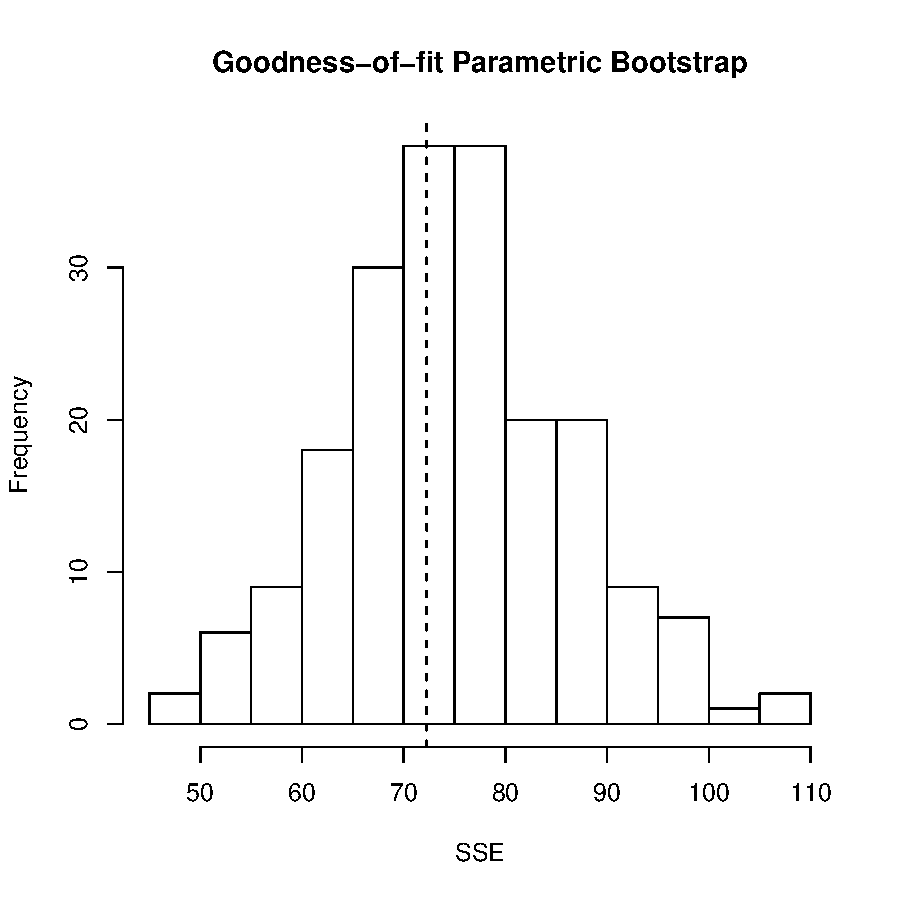
\includegraphics{unmarked-034}
\caption{Examine estimated abundance for Ovenbird removal data.  Band
  is 95\% confidence interval.}
\label{fig:pred}
\end{figure}


Next, we organize the fitted models with the \code{fitList} function and
the use the \code{modSel} method to rank the models by AIC.



\begin{Schunk}
\begin{Sinput}
R> fmList <- fitList(`lam(ufp+trba)p(.)` = fm.oven.1, 
+     `lam(ufp*trba)p(.)` = fm.oven.2, `lam(ufp)p(.)` = fm.oven.3, 
+     `lam(trba)p(.)` = fm.oven.4, `lam(.)p(.)` = fm.oven.5)
R> modSel(fmList)
\end{Sinput}
\begin{Soutput}
                  nPars    AIC delta AICwt cumltvWt
lam(trba)p(.)         3 324.77  0.00  0.35     0.35
lam(ufp)p(.)          3 325.73  0.96  0.21     0.56
lam(ufp+trba)p(.)     4 326.14  1.37  0.17     0.73
lam(.)p(.)            2 326.28  1.51  0.16     0.90
lam(ufp*trba)p(.)     5 327.17  2.40  0.10     1.00
\end{Soutput}
\end{Schunk}



\code{predict} functions much like \code{linearComb} except that new data can be
passed to it as a \code{data.frame} rather than a design matrix. When the first
argument given to predict is a list of models created by \code{fitList},
\code{predict} computes model-averaged predictions, which may be
useful in the presence of high model selection uncertainty.



\subsection{Goodness of fit and the parametric bootstrap}

To conduct goodness of fit tests, \um\ provides a generic parametric
bootstrapping function \code{parboot}.  It simulates data from the fitted model and
applies a user-defined function that returns a fit-statistic such as the
Pearson's $\chi^2$.



\begin{figure}[th!]
  \centering
\includegraphics{unmarked-039}
\caption{Graphical assessment of model fit by parametric bootstrapping.  The dashed
line is the observed chi-squared statistic. The histogram approximates the
expected sampling distribution.}
\label{fig:pb}
\end{figure}

\begin{Schunk}
\begin{Sinput}
R> set.seed(1234)
R> chisq <- function(fm) {
+     observed <- getY(fm@data)
+     expected <- fitted(fm)
+     sum((observed - expected)^2/expected)
+ }
R> pb <- parboot(fm.oven.1, statistic = chisq, nsim = 200)
\end{Sinput}
\end{Schunk}
\begin{Schunk}
\begin{Sinput}
R> plot(pb, main = "")
\end{Sinput}
\end{Schunk}


The above call to \code{plot} with a parametric bootstrap object as
the argument produces a useful graphic for assessing goodness of fit
(Figure~\ref{fig:pb}).  The plot suggests that the model adequately
explains these data.

Beyond serving as a tool to evaluate goodness of fit,
\code{parboot} can be used to characterize uncertainty in any derived quantity
of interest.


\section[Future directions for unmarked development]{Future directions for \um\ development}
\label{sec:future-direct-unmark}

\um\ has become a stable and useful platform for the analysis of ecological
data, but several areas of development could improve its utility.  First, new
models need to be added to cover the range of sampling techniques and
population dynamics commonly encountered. Table~\ref{tab:modspace} illustrates
some of the gaps that need to be filled. In most cases, models to fill these
gaps have not been developed so more research is needed.


Second, each of the models in \um\ assumes independence among sites. However,
ecologists often use sampling methods such as cluster sampling that induce
spatial dependence. Typically, this is done for logistical convenience, but
because few methods are available to account for spatial correlation and
imperfect detection probability, the spatial dependence is often ignored.
Rather than this being a weakness of the sampling design, we envision that
this dependence can be used as information regarding the spatial distribution
of individuals.

Third, many of the likelihoods are written in pure \rlang, which can be
slow for large problems. We are currently translating many of these
functions into \proglang{C++} with the help of the R package \pkg{Rcpp}
\citep{Rcpp11}.

Finally, Markov chain Monte Carlo methods could be implemented for all
of these models allowing for Bayesian inference.  An
important advantage of Bayesian analysis over classical methods is that the
latent abundance or occurrence variables can be treated as formal parameters.
Thus posterior distributions could easily be calculated for derived parameters
such as the proportion of sites occupied.  Bayesian analysis also would provide
a natural framework for incorporating additional sources of random variation.
For example, one could model heterogeneity among sites not accounted for by
covariates alone.

\begin{table}[bt] %\small
\begin{centering}
\begin{tabular}{lccc}
\hline
Sampling method & \multicolumn{3}{c}{Population Dynamics} \\
\cline{2-4}
                            & Closed              & Open to         & Open to \\
                            &                     & temporary       & demographic \\
                            &                     & emigration      & processess \\
\hline
Occurrence sampling         & \code{occu}         & ---             & \code{colext} \\
Repeated counts             & \code{pcount}       & ---             & \code{pcountOpen} \\
Removal sampling, \\double observer sampling,  & \code{multinomPois}& \code{gmultmix}  & --- \\
and other multinomial designs \\
Distance sampling           & \code{distsamp}     & ---               & --- \\
\hline
\end{tabular}
\caption{Model fitting functions classified by sampling method and population
dynamics. Missing cells indicate models that have not been developed but are
likely to be investigated in the future.}
\label{tab:modspace}
\end{centering}
\end{table}

\newpage

\section*{Acknowledgements}

The authors thank Andy Royle of the United States Geological Survey's
Patuxent Wildlife Research Center, who provided initial funding and
inspiration for this work. Andy Royle and Robert Dorazio made valuable
suggestions that greatly improved an earlier version of the manuscript.

%%\bibliographystyle{jss}
\bibliography{unmarked}

\end{document}
